%***********************************************************************
\subsection{Calibration Evaluation}\label{sub:bc_calibration_evaluation}
%***********************************************************************

% FEBA Test No. 216 Posterior w/ bias term Uncertainty Propagation, TC
\clearpage
\begin{sidewaysfigure}
	\centering
	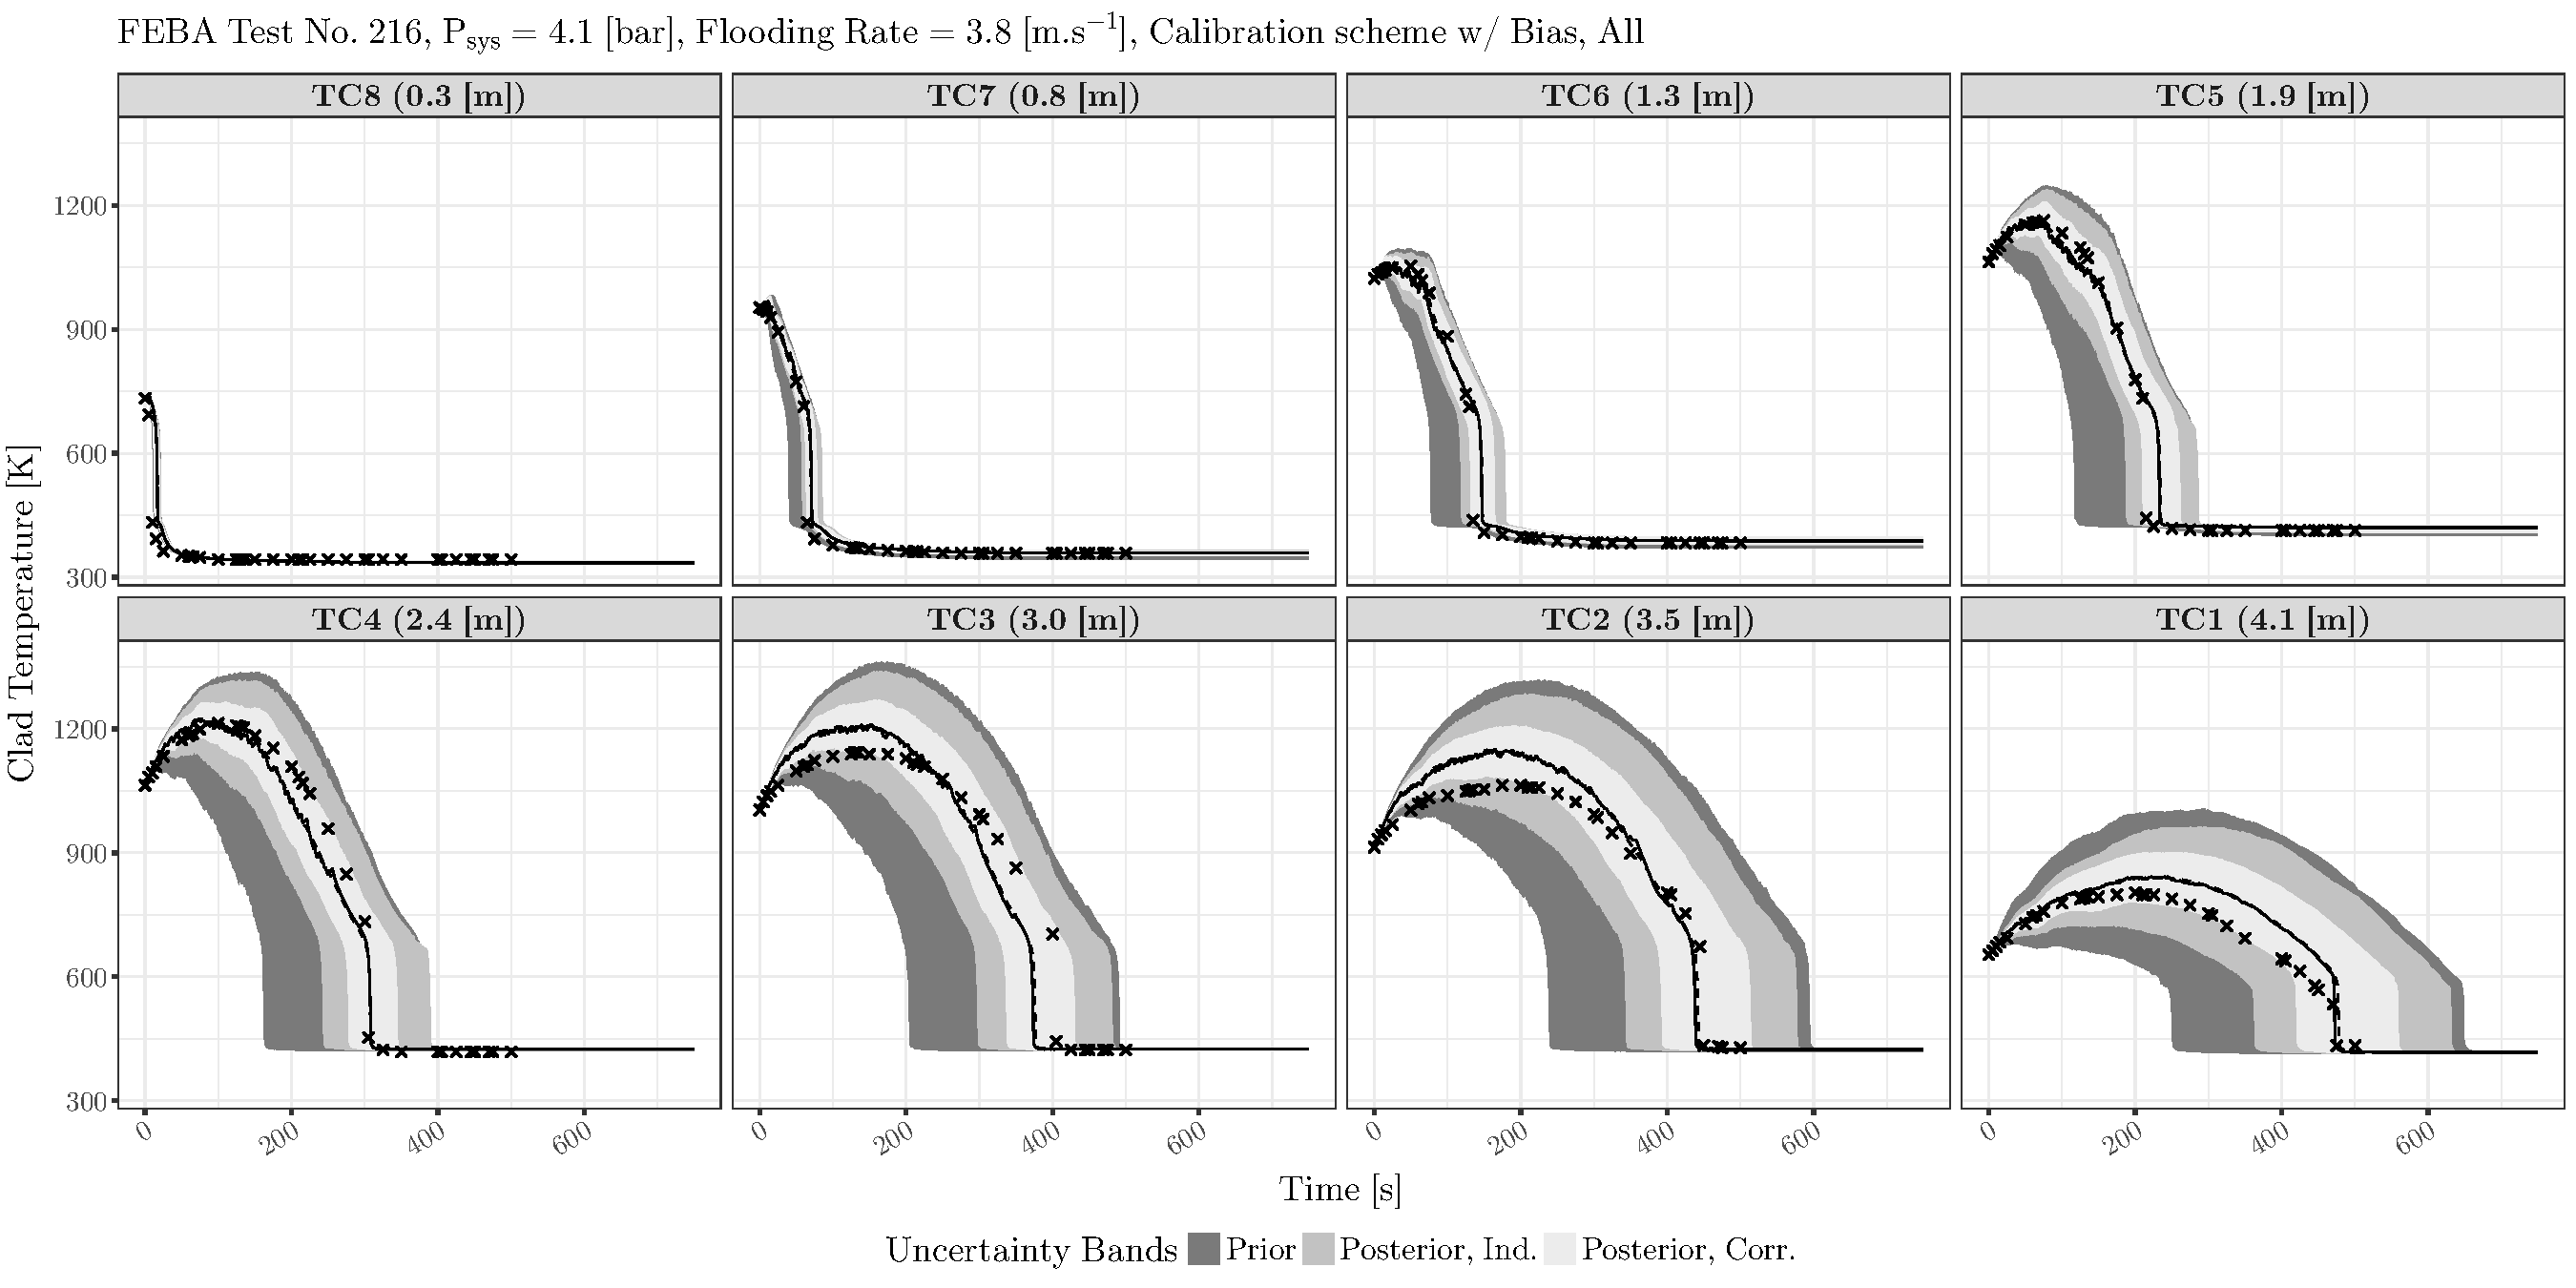
\includegraphics[width=0.90\textwidth]{../figures/chapter5/figures/plotTraceUQPosteriorAllDiscCenteredTC216}
		\captionof{figure}[Posterior uncertainty propagation of FEBA Test No. $216$ for the cladding temperature output ($TC$). Calibration with model bias term.]{Uncertainty propagation of the parameters uncertainty of \gls[hyper=false]{feba} Test No. $216$ for the cladding temperature output ($TC$) at different axial locations. The uncertainty bounds refer to the symmetric ($95\%$) probability: dark gray, gray, and light gray correspond to the prior, correlated posterior, and independent posterior samples of the parameters, respectively. Solid lines, dashed lines, and crosses indicate the simulation with the nominal parameters values, the median of the posterior uncertainties, and the experimental data, respectively. Posterior samples from calibration with model bias term.}
	\label{fig:ch5_plot_trace_uq_post_tc_216_disc}
\end{sidewaysfigure}
\clearpage

% FEBA Test No. 216 Posterior w/ bias term Uncertainty Propagation, DP
\bigfigure[pos=tbhp,
           opt={width=1.0\textwidth},
           label={fig:ch5_plot_trace_uq_post_dp_216_disc},
           shortcaption={Posterior uncertainty propagation of FEBA Test No. $216$ for the pressure drop output ($DP$). Calibration with model bias term.}]
{../figures/chapter5/figures/plotTraceUQPosteriorAllDiscCenteredDP216}
{Uncertainty propagation of the parameters uncertainty of \gls[hyper=false]{feba} Test No. $216$ for the cladding temperature output ($TC$) at different axial locations. The uncertainty bounds refer to the symmetric ($95\%$) probability: dark gray, gray, and light gray correspond to the prior, correlated posterior, and independent posterior samples of the parameters, respectively. Solid lines, dashed lines, and crosses indicate the simulation with the nominal parameters values, the median of the posterior uncertainties, and the experimental data, respectively. Posterior samples from calibration with model bias term.}

% FEBA Test No. 216 Posterior w/ bias term Uncertainty Propagation, CO
\begin{figure}[!bth]
    \centering
    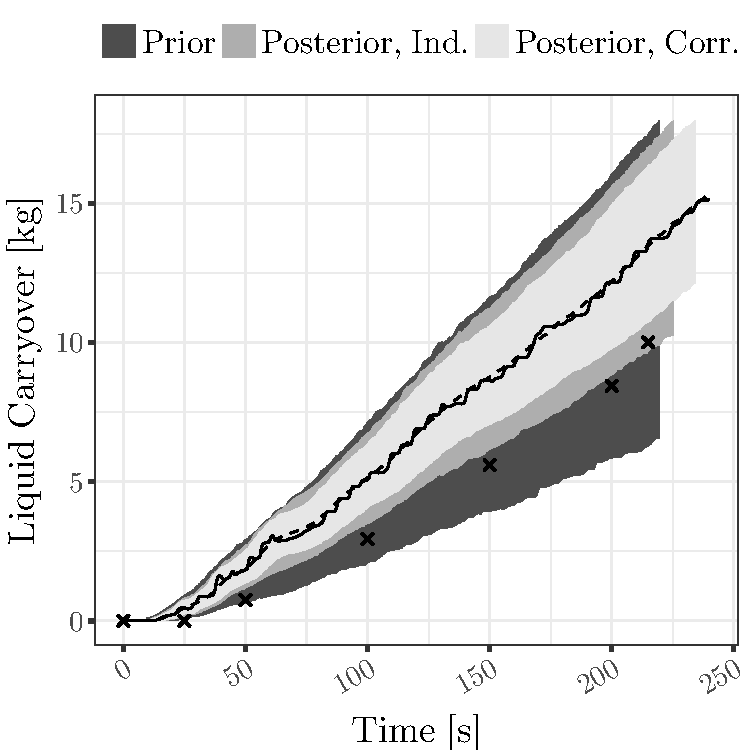
\includegraphics[width=0.5\textwidth]{../figures/chapter5/figures/plotTraceUQPosteriorAllDiscCenteredCO216}
    \caption[Posterior uncertainty propagation of FEBA Test No. $216$ for the liquid carryover output ($CO$). Calibration with model bias term.]{Uncertainty propagation of the parameters uncertainty of \gls[hyper=false]{feba} Test No. $216$ for the cladding temperature output ($TC$) at different axial locations. The uncertainty bounds refer to the symmetric ($95\%$) probability: dark gray, gray, and light gray correspond to the prior, correlated posterior, and independent posterior samples of the parameters, respectively. Solid lines, dashed lines, and crosses indicate the simulation with the nominal parameters values, the median of the posterior uncertainties, and the experimental data, respectively. Posterior samples from calibration with model bias term.}
    \label{fig:ch5_plot_trace_uq_post_co_216_disc}
\end{figure}

% Calibration Score vs Informativeness
\clearpage
\begin{sidewaysfigure}
	\centering
	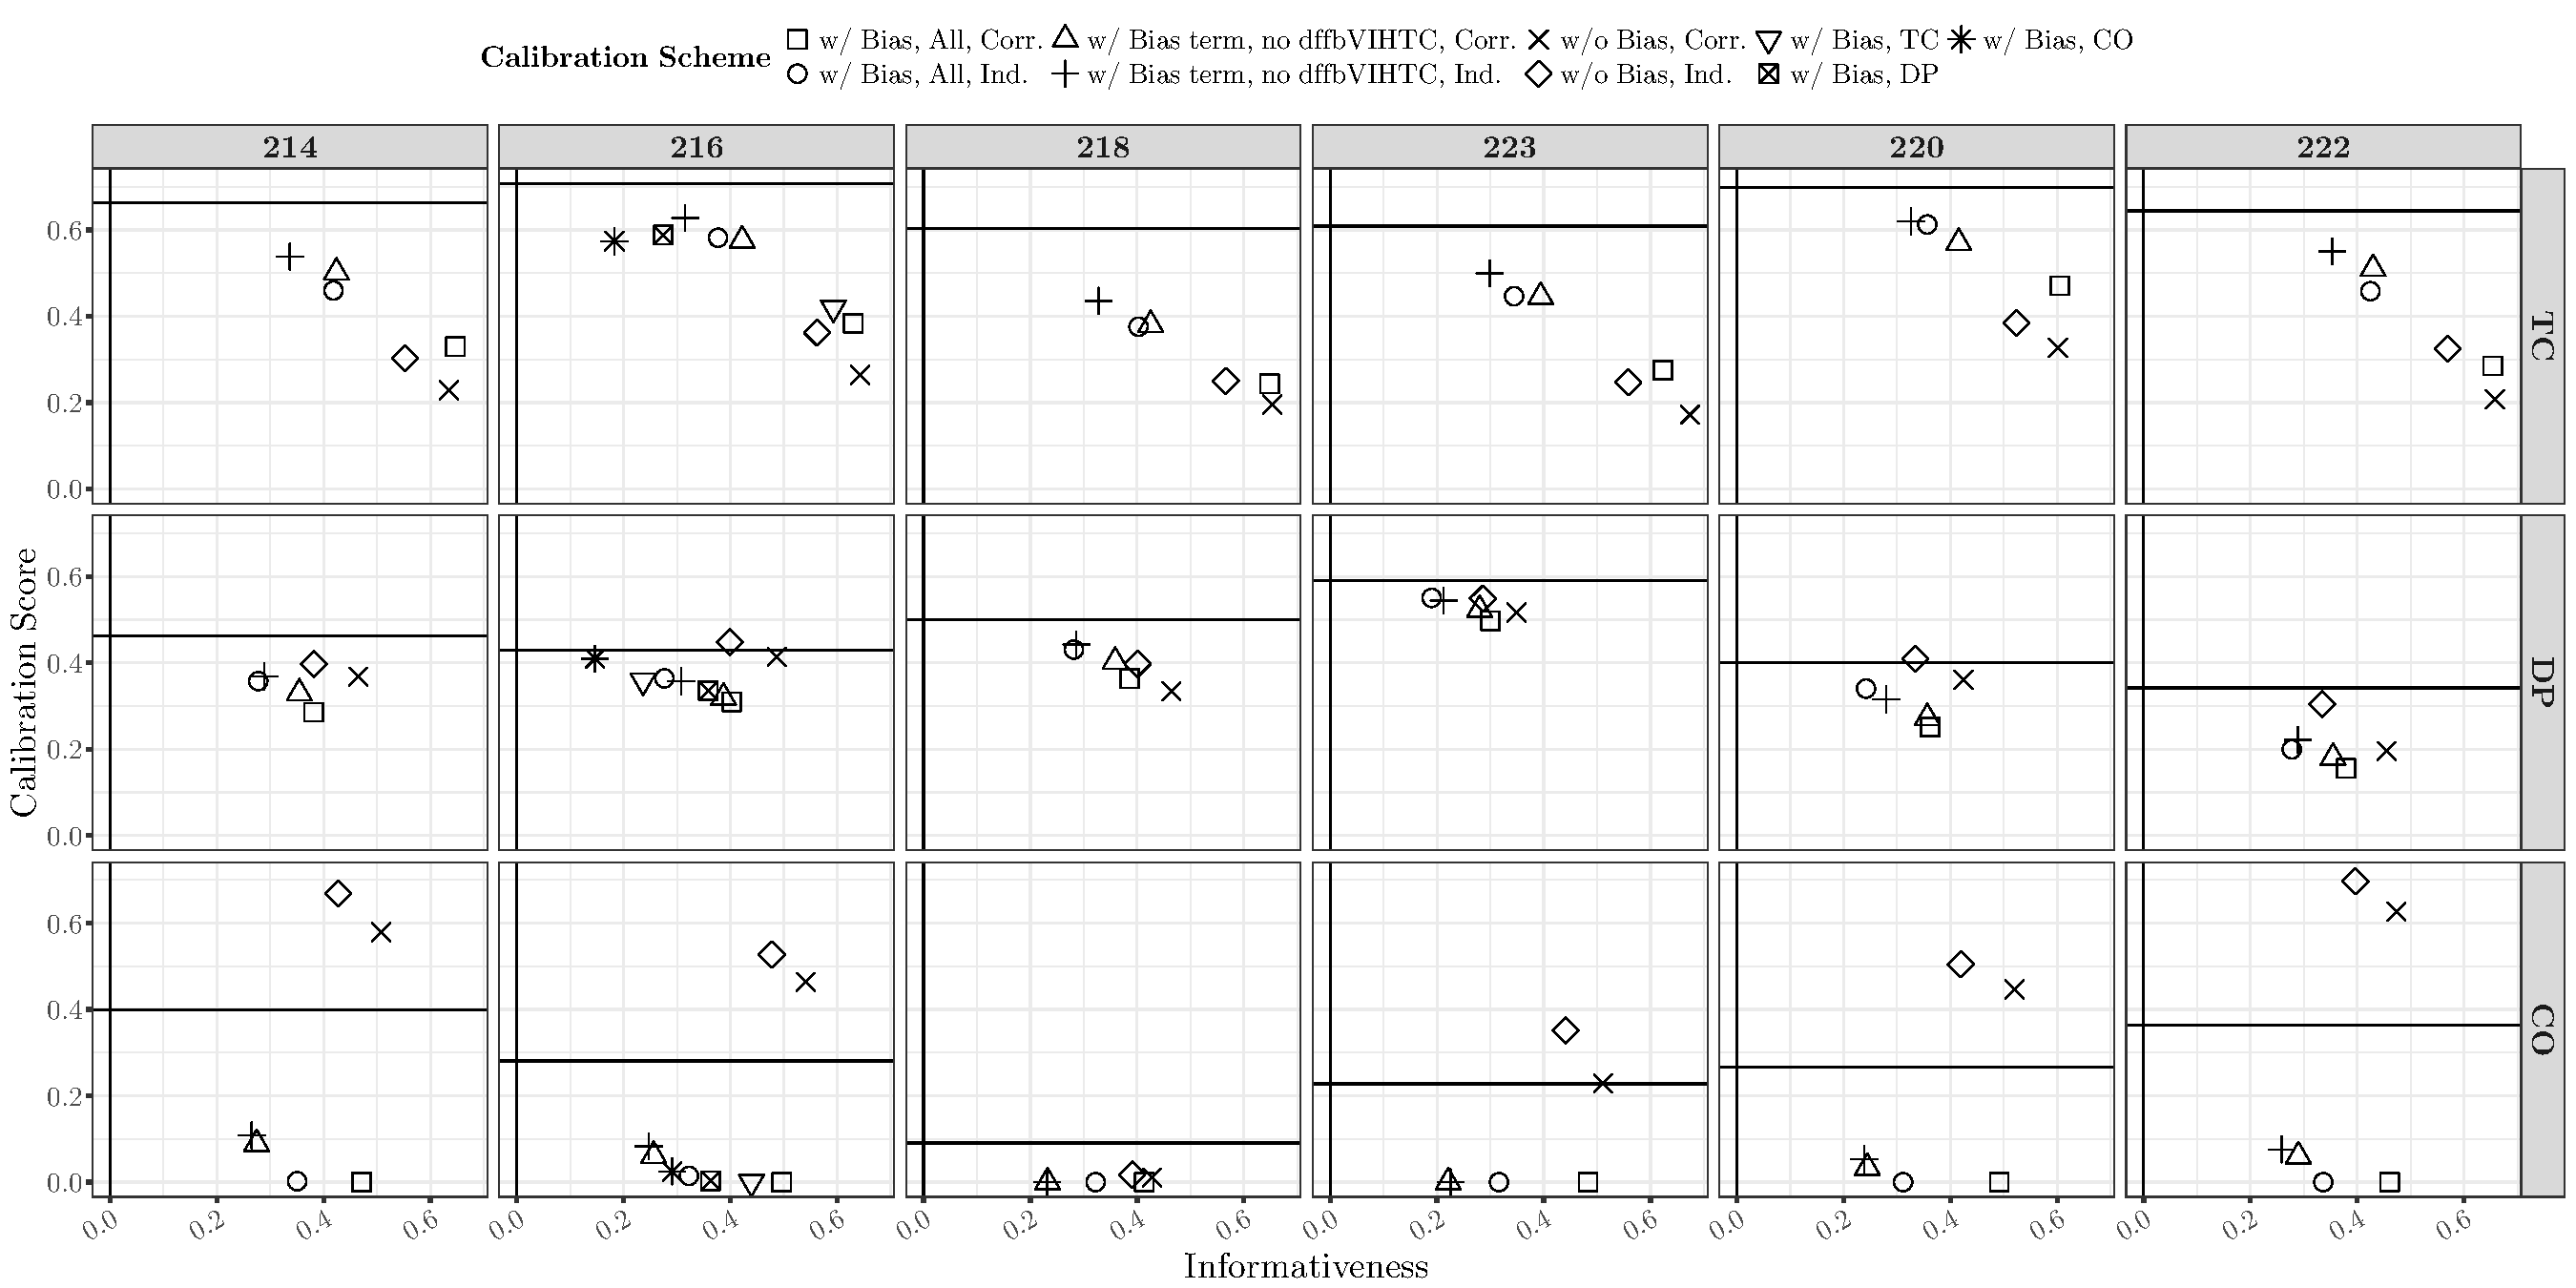
\includegraphics[width=0.95\textwidth]{../figures/chapter5/figures/plotCalibInfo}
		\captionof{figure}[Calibration score vs. Informativeness for different posterior samples propagated on all the FEBA tests.]{Calibration score vs. Informativeness for different posterior samples propagated on all the gls[hyper=false]{feba} tests. Vertical lines indicate the informativeness of the prior uncertainty (defined as $0$) while the horizontal lines indicate the initial Calibration score (i.e., that of the prior).}
	\label{fig:ch2_plot_trace_uq_prior_tc_218}
\end{sidewaysfigure}
\clearpage


